\documentclass[runningheads]{llncs}
\usepackage{xcolor}
\usepackage{listings} 
\usepackage{graphicx}


\usepackage{graphicx}


\usepackage[utf8]{inputenc} %Together with 'spanish' package, allows you to write accents 

%This package allows the use of accents, the parameter 'es-tabla' writes Tabla instead of 'Cuadro', the parameter es-noindentfirst makes that the first line after each section and subsection is not indented
\usepackage[spanish,activeacute,es-tabla,es-noindentfirst]{babel}

%This package allows you among other things, use as option [H] in tables and figures, which set the object just where you put in the source code.
\usepackage{float}

%This package allows you to write pseudocode, you should read the docummentation to use it properly 
\usepackage{algorithm2e}

%Packages to write math
\usepackage{amssymb}
\usepackage{amsmath}

%permite el formato de múltiple citación agrupada dentro de los corchetes
\usepackage{cite} 

\usepackage{times}
\usepackage{color}

%Package that help to write text that will appear like you write in the final documment
\usepackage{verbatim}

%This package allows you to configure tables and figures
\usepackage{caption}

%Package to customize formats to the tables
\usepackage{booktabs}

%Package to control hiperlinks
\usepackage[breaklinks=true]{hyperref}
\hypersetup{
	colorlinks=true,
	linkcolor=blue,
	filecolor=magenta,      
	urlcolor=blue,
	citecolor=cyan,
}

%Package to stablish the margins of the documment
\usepackage{vmargin}

%A0, A1, ..., A9, B0, B1, ..., B9, C0, ..., C9, USletter, USlegal, and USexecutive
\setpapersize{A4}
%\setmarginsrb{hleftmargini}{htopmargini}{hrightmargini}{hbottommargini}%
%{hheadheighti}{hheadsepi}{hfootheighti}{hfootskipi}

\setmarginsrb{30mm}{25mm}{30mm}{25mm}{6mm}{7mm}{5mm}{15mm}

%También puede utilizar esta sintaxis para establcer los márgenes con el paquete {vmargin}
%\setmargins{3.0cm}       % margen izquierdo
%{1.5cm}                        % margen superior
%{14.5cm}                      % anchura del texto
%{23.42cm}                    % altura del texto
%{10pt}                           % altura de los encabezados
%{1cm}                           % espacio entre el texto y los encabezados
%{0pt}                             % altura del pie de página
%{2cm}         

%Estos paquetes se utilian para escribir psudocódigo, sin embargo en estos momentos se está utilizando el paquete {algorithm2e}
%\usepackage{algpseudocode}
%\usepackage{algorithmicx}
%\usepackage{algorithm}

\definecolor{gray97}{gray}{.97}
\definecolor{gray75}{gray}{.75}
\definecolor{gray45}{gray}{.45}

%Packages to write code in various programming languajes, please, see the docummentation 
\usepackage{listings}
\usepackage{listingsutf8}
\lstset{frame=Ltb,
	framerule=0pt,
	aboveskip=0.5cm,
	framextopmargin=3pt,
	framexbottommargin=3pt,
	framexleftmargin=0.4cm,
	framesep=0pt,
	rulesep=.4pt,
	backgroundcolor=\color{gray97},
	rulesepcolor=\color{black},
	%
	stringstyle=\ttfamily,
	showstringspaces = false,
	basicstyle=\small\ttfamily,
	commentstyle=\color{blue},
	keywordstyle=\bfseries,
	%
	numbers=left,
	numbersep=15pt,
	numberstyle=\tiny,
	numberfirstline = false,
	breaklines=true,
}
\lstnewenvironment{listing}[1][]
{\lstset{#1}\pagebreak[0]}{\pagebreak[0]}

\lstdefinestyle{consola}
{basicstyle=\scriptsize\bf\ttfamily,
	backgroundcolor=\color{gray75},
}
\lstdefinestyle{C}
{language=C,
}
% Used for displaying a sample figure. If possible, figure files should
% be included in EPS format.
%
% If you use the hyperref package, please uncomment the following line
% to display URLs in blue roman font according to Springer's eBook style:
\renewcommand\UrlFont{\color{blue}\rmfamily}

%\renewcommand\Algorithmname{Algoritmo}
\renewcommand\examplename{Ejemplo}
\renewcommand\exercisename{Ejercicio}
\renewcommand\figurename{Fig.}
\renewcommand\keywordname{{\bf T\'erminos Clave:}}
\renewcommand\indexname{Index}
\renewcommand\lemmaname{Lema}
\renewcommand\contriblistname{Lista de colaboradores}
\renewcommand\listfigurename{Lista de Figuras}
\renewcommand\listtablename{Lista of Tablas}
\renewcommand\mailname{{\it Correspondencia para\/}:}
\renewcommand\noteaddname{Note added in proof}
\renewcommand\notename{Nota}
\renewcommand\partname{Parte}
\renewcommand\problemname{Problema}
\renewcommand\proofname{Demostración}
\renewcommand\propertyname{Propiedad}
\renewcommand\propositionname{Proposici\'on}
\renewcommand\questionname{Pregunta}
\renewcommand\remarkname{Remark}
\renewcommand\seename{Ver}
\renewcommand\solutionname{Soluci\'on}
\renewcommand\theoremname{Teorema}
\begin{document}


\section{}
\section{}
\section{\centering{Desarrollo}}
\subsection{Análisis de requerimientos.}

\subsubsection{Requerimientos Funcionales}
\begin{itemize}
    \item \textbf{Validacion del Usuario}
    \begin{itemize}
        \item \textbf{Registro de Usuario: }El sistema requerirá que los usuarios se registren en el sistema proporcionando su información de identificación, como su clave de colportor, correo electrónico y contraseña. Este proceso permitirá la validación de la identidad del usuario y el acceso al sistema. Además, el registro también permitirá al sistema recopilar información adicional, como su Nombre Completo, Teléfono y Dirección en el campo asignado. Esta información puede ser utilizada por el sistema para establecerla como información del vendedor al momento de emitir el comprobante de venta.
        \item \textbf{Inicio de Sesión: }El proceso de inicio de sesión permitirá a los usuarios acceder al sistema ingresando su información de acceso validada en el proceso de registro. El sistema verificará la información de acceso proporcionada por el usuario y le dará acceso a las funciones del sistema. Además, el sistema también puede implementar medidas de seguridad a nivel de servidor para validar la información de ingreso del usuario como el cifrado de contraseña.
    \end{itemize}    
    \item \textbf{Pantalla de Inicio: }
    La pantalla de inicio del sistema de gestión de colportaje mostrará información relevante al usuario, como el total de libros vendidos, el total de diezmo que debe entregar a la asociación en base a las ventas, la cantidad de pedidos pendientes y el total de ventas realizadas. También se mostrará un resumen de los pedidos realizados y el estado actual de cada uno, es decir, si están pendientes de entrega o entregados. Esta información permitirá al usuario tener un panorama general del estado de sus ventas y pedidos, así como de su desempeño en el colportaje.
    \item \textbf{Gestión de Ventas}
    \begin{itemize}
        \item \textbf{Registro de Venta: }El registro de venta permitirá a los usuarios registrar los detalles de cada venta realizada en el sistema de colportaje. Para ello, se deberá ingresar la información de venta, como la fecha del pedido y la fecha de entrega, la selección del material que incluye: el título de las obras solicitadas, la cantidad de libros solicitados de cada titulo y su correspondiente precio y marcar si el material fue entregado o no. También se deberá registrar la información del cliente. En caso de que la venta se haya realizado a crédito, se deberá registrar el pago inicial y el saldo a pagar, así como la cantidad de pagos y su frecuencia. Además, de la información del colportor que realiza la venta y el precio final de venta y la firma del cliente.
        \item \textbf{Información del Cliente: }La información del cliente incluirá detalles sobre el nombre, dirección, correo electrónico y teléfono del cliente. Además, el sistema también puede incluir opciones de personalización para que los usuarios puedan agregar detalles adicionales sobre cada cliente, como una referencia de su ubicación o alguna nota adicional del cliente.
        \item \textbf{Información de Pago: }La información de pago incluirá detalles sobre el pago inicial y el saldo a pagar en caso de que la venta se haya realizado a crédito, así como la cantidad de pagos y sus fechas. Además, se podrá registrar cada pago que se realice de acuerdo a las fechas de cobro establecidas.
        \item \textbf{Información del Colportor: }La información del colportor se incluye en base al talonario de venta que se utiliza actualmente, y se toma de la información ingresada al momento de hacer el registro de usuario.
    \end{itemize}    
    \item \textbf{Gestión de Clientes y Referencias}
    \begin{itemize}
        \item \textbf{Registrar nuevo cliente: }El registro de nuevo cliente permitirá a los usuarios registrar la información personal de nuevos clientes, como su nombre, teléfono y dirección. El registro del cliente se realiza al momento de hacer una venta o levantar un pedido.
        \item \textbf{Consultar Clientes y Referencias: }La consulta de clientes actuales permitirá a los usuarios acceder a una lista de los clientes registrados en el sistema de colportaje.
        \item \textbf{Gestión de Referencias: }La gestión de referencias permitirá a los usuarios registrar referencias de clientes y validar si se ha visitado o si está pendiente por visitar. Esto permitirá a los usuarios planificar y organizar sus visitas a las referencias de manera más eficiente y efectiva.
    \end{itemize}    
    \item \textbf{Inventario y Selección de Libros}
    \begin{itemize}
        \item \textbf{Registrar los libros comprados a la editorial (contado o crédito): }El inventario del sistema de colportaje permitirá al usuario registrar los libros disponibles para la venta. Para ello, se deberá registrar el título de los libros, su precio de venta, el precio de compra a la editorial y la cantidad disponible en el inventario. El sistema permitirá al usuario consultar el catálogo de libros disponibles, así como el estado del inventario, es decir, la cantidad de libros disponibles y los que están en proceso de venta. El sistema también permitirá al usuario registrar las compras realizadas a la editorial, ya sea de contado o a crédito, y llevar un historial de las deudas pendientes por pagar.
        \item \textbf{Consultar Libros: }La consulta de libros permitirá a los usuarios acceder a una lista de los libros disponibles para la venta así como su precio. 
    \end{itemize}    
\end{itemize}
\subsubsection{Requerimientos No Funcionales}
Algunos de los requerimientos no funcionales que son necesarios para este proyecto incluyen:
\begin{itemize}
    \item \textbf{Usabilidad: } El software debe ser fácil de usar e intuitivo para los colportores sin experiencia previa en tecnología. La interfaz debe ser clara y sencilla, y el software debe ser capaz de realizar tareas complejas de manera fácil y sin confusiones.
    \item \textbf{Escalabilidad: } El software debe ser escalable y capaz de manejar un gran volumen de datos y transacciones a medida que el club de colportores crece y se expande.
    \item \textbf{Seguridad: } El software debe ser seguro y proteger la información del usuario, como los datos de venta y los detalles de pago, de posibles amenazas de seguridad.
    \item \textbf{Disponibilidad: } El software debe estar disponible para su uso en todo momento, ya que los colportores pueden necesitar acceder a él en cualquier momento y lugar.
    \item \textbf{Rendimiento: }El software debe ser rápido y eficiente, y ser capaz de manejar grandes cantidades de datos sin afectar el rendimiento general del sistema.
    \item \textbf{Compatibilidad: } El software debe ser compatible con una variedad de dispositivos y sistemas operativos para garantizar que los colportores puedan acceder a él desde cualquier dispositivo que tengan disponible.
    \item \textbf{Mantenimiento: } El software debe ser fácil de mantener y actualizar, y debe incluir herramientas de monitoreo y diagnóstico para ayudar a la identificación y solución de problemas.
    \item \textbf{Integración: } El software debe ser capaz de integrarse con otros sistemas y herramientas utilizados por el club de colportores, como sistemas de contabilidad o de seguimiento de inventario, para garantizar una mayor eficiencia y coordinación en el proceso de colportaje.
\end{itemize}
\subsection{Diagramas de Flujo.}
Los diagramas de flujo son una herramienta importante para visualizar el proceso de gestión de colportaje propuesto. Estos muestran las fases necesarios para completar cada tarea en el proceso, lo que permite a los desarrolladores identificar áreas de mejora y optimización. Además, son útiles para capacitar a los usuarios finales en el uso del software.

Cada flujo de la aplicación se describe en los diagramas, con el fin de entender cada proceso a realizar dentro de la aplicación y los pasos a seguir para ejecutar alguna tarea especifica.

Dentro de los principales flujos del software propuesto, se describen los siguientes:

\subsection*{Proceso de Venta}
Es el proceso principal dentro del sistema. Comprende todo el proceso de realizacion de una venta y la informacion necesaria para su registro (ver Figura \ref{fig1}).
Esta compuesto tanto por el proceso principal de registro de venta como de algunos subprocesos definidos mas adelante.
El flujo que se sigue se especifica de la siguiente manera:
\begin{enumerate}
    \item Se registra la fecha del pedido
    \item Selecciona el tipo de venta 
    \item Se realiza la seleccion del material (Subproceso)
    \item Se registra la fecha de entrega del material
    \item Ingresa el costo total de la venta
    \item Registro del pago inicial o total
    \item Registro de la informacion del cliente (Subproceso)
    \item Registrar firma del cliente
    \item Se obtienen los datos del colportor
    \item Se emite el recibo de venta
\end{enumerate}
%TODO: Cambiar orientacion
\begin{figure}[H]
	\centering\captionsetup{width=0.8\textwidth}
	\includegraphics[width=1\textwidth]{figures/diagramas_de_flujo/Flujo de Registro _ Realización de una venta.png}
	\caption{Diagrama de Flujo de Registro de Ventas} \label{fig1}
\end{figure}

\subsection*{Proceso de Seleccion de Libros}
En la Figura \ref{fig2} se observa el flujo del proceso de selección de libros.
Este se inicia ejecutando una validación para identificar el tipo de transaccion que se esta realizando para llevar a cabo la selección de los libros, ya sea una compra para registrar un credito o una venta a un cliente.
En base al tipo de transaccion seleccionado se asigna un precio de los materiales a la hora de su seleccion y se muestran en una lista dinamica.
A partir de aqui, el flujo se desprende en tres elementos para la seleccion: El primero busca un material en especifico, en donde se ingresa el titulo del material deseado y se procede con la seleccion. El segundo realiza la seleccion directamente de la lista de libros que se muestra. El tercero muestra mas informacion sobre los libros como su descripcion, autor, etc.
Conforme se seleccionan los libros, en la barra superior de la pantalla se vera reflejado el costo acumulativo de los materiales que se seleccionen, con el objetivo de que el colportor tenga una referencia del costo total que podria asignar al pedido. Esto ultimo en caso de que el tipo de transaccion sea una venta.
Una vez seleccionado el material se concluye el flujo agregando la cantidad a solicitar de cada libro seleccionado.
\begin{figure}[H]
	\centering\captionsetup{width=0.8\textwidth}
	\includegraphics[width=1\textwidth]{figures/diagramas_de_flujo/Flujo de Selección de Material (Libros).png}
	\caption{Diagrama de Flujo de Selección de Libros} \label{fig2}
\end{figure}


\subsection*{Proceso de Registro de Clientes y Referencias}
Dentro del flujo de este subproceso esta especificada la informacion que se requiere tanto de los clientes (ver Figura \ref{fig3}) como de las referencias (ver Figura \ref{fig4}) del colportor.
Si bien, el proceso es similar entre ambos subprocesos, existen algunas validaciones que se ejecutan durante el flujo y registro de informacion.

En el flujo de registro de cliente se valida que al registrarlo sea una referencia o no, ya que si se ha registrado como referencia, unicamente se completa la informacion faltante del cliente. 
Ademas de validar que la informacion ingresada este completa y no tenga algun error.

Por otro lado, el flujo de registro de referencia, ademas del registro de informacion de la referencia, se valida que aun no haya sido visitado anteriormenete.

\begin{figure}[H]
	\centering\captionsetup{width=0.8\textwidth}
	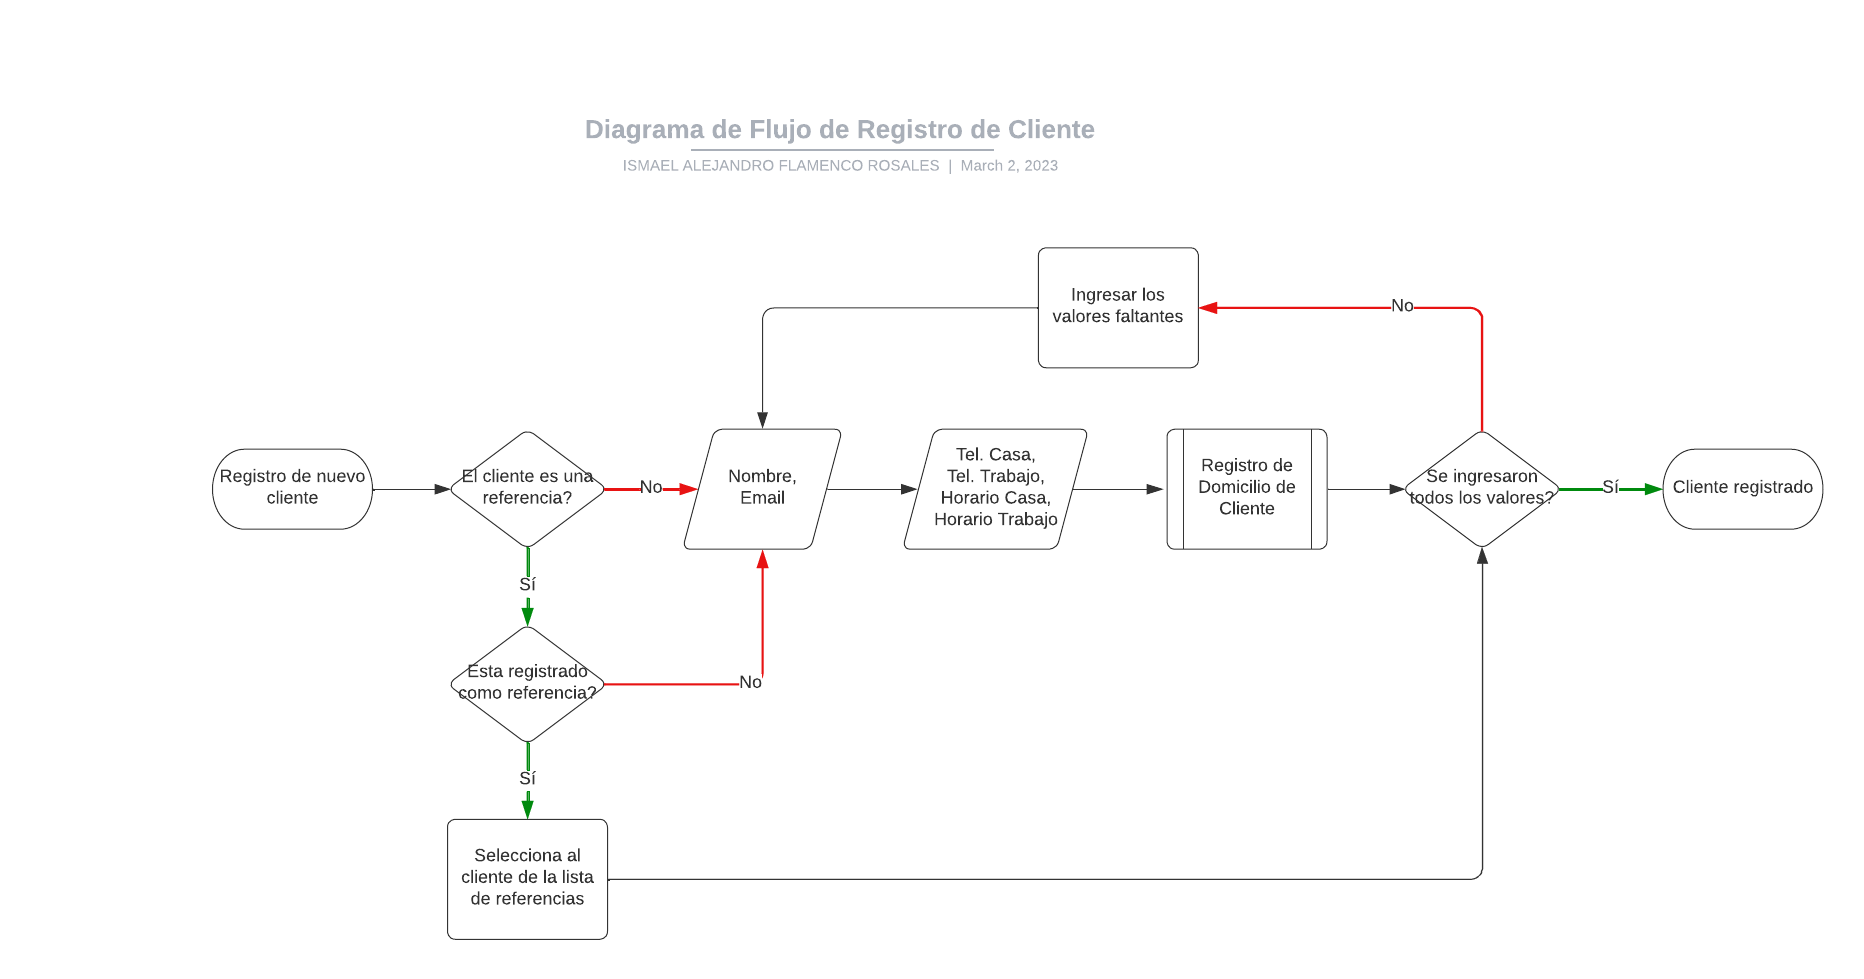
\includegraphics[width=1\textwidth]{figures/diagramas_de_flujo/Flujo de Registro de Cliente.png}
	\caption{Diagrama de Flujo de Registro de Clientes} \label{fig3}
\end{figure}
\begin{figure}[H]
	\centering\captionsetup{width=0.8\textwidth}
	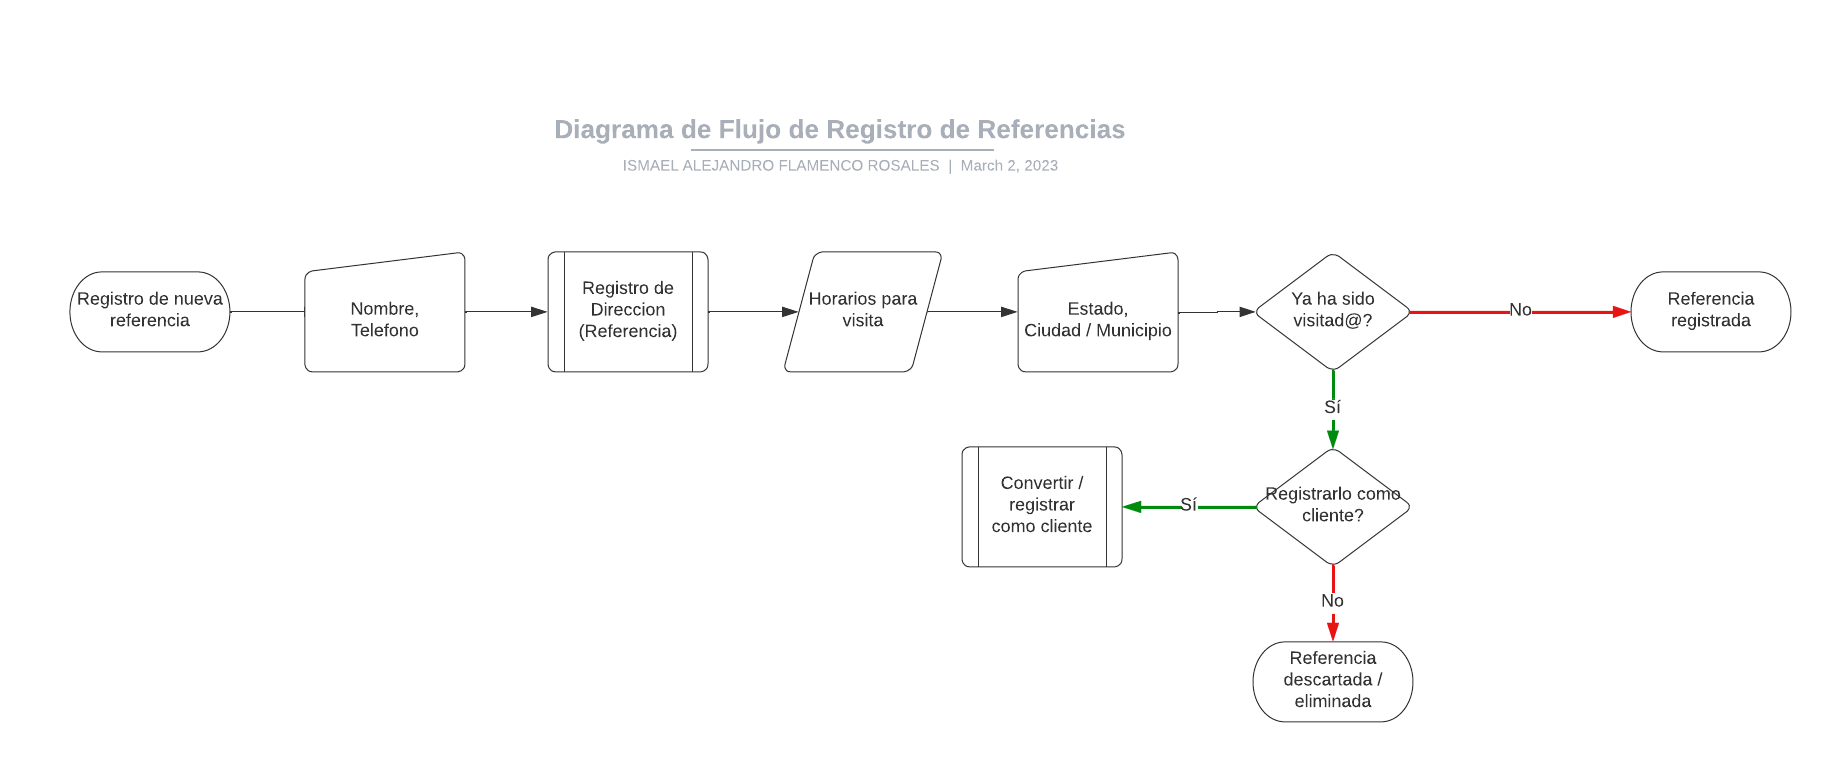
\includegraphics[width=1\textwidth]{figures/diagramas_de_flujo/Flujo de Registro de Referencias.png}
	\caption{Diagrama de Flujo de Registro de Referencias} \label{fig4}
\end{figure}

\subsection{Esquema conceptual y Diseño de la Base de Datos.}
Dentro del esquema conceptual de la base de datos se especifican aquellos componentes o elementos principales que interactuan con la base de datos.
La interacción y relacion entre ellos dependera de su funcionalidad, y como podemos observar en la Figura \ref{fig5} se muestra graficamente la interacción entre dichos componentes, la cual se describe de la siguiente manera:

\subsection*{Controlador de Creditos}
Es el componente de la aplicación que se encarga de gestionar los créditos otorgados a los clientes. Este componente se comunica con el subsistema de gestión de ventas para obtener información sobre las ventas realizadas y con el subsistema de seguridad para autenticar y autorizar las solicitudes de crédito.

También se comunica con el subsistema de pagos, para registrar los pagos de los clientes y actualizar el estado de los créditos. Por último, este componente se comunica con el subsistema de bonificaciones, para aplicar las bonificaciones correspondientes a los clientes.

\subsection*{Subsistema de Seguridad}
Se encarga de autenticar y autorizar las solicitudes de los usuarios. Este subsistema está compuesto por los siguientes componentes:
\begin{itemize}
    \item \textbf{Autenticación de Usuario:}  Este servicio es responsable de autenticar a los usuarios de la aplicación.
    \item \textbf{Autorización de Usuario:} Es responsable de autorizar las solicitudes de los usuarios de la aplicación.
\end{itemize}

\subsection*{Subsistema de Pagos}
Gestiona los pagos de los clientes. Está compuesto por los siguientes componentes:
\begin{itemize}
    \item \textbf{Registro de Pago:}  Es responsable de registrar los pagos de los clientes.
    \item \textbf{Consulta de Pagos:} Es responsable de consultar los pagos realizados por los clientes.
\end{itemize}
El subsistema de pagos se comunica con el controlador de créditos para registrar los pagos de los clientes y actualizar el estado de los créditos.
\subsection*{Subsistema de Bonificaciones}
Determina el total a recibir en base a las bonificaciones establecidas previamente (21\% por parte de GEMA y 14\% por parte de la Universidad) y respecto a las ventas realizadas por parte del colportor.
\subsection*{Interfaz de Pedidos}
Permite a los colportores registrar y gestionar sus pedidos. Esta interfaz está compuesta por los siguientes componentes:
\begin{itemize}
    \item \textbf{Formulario de Registro de Pedidos:}  Permite a los colportores registrar sus pedidos.
    \item \textbf{Lista de Pedidos:} Muestra la lista de pedidos registrados por los colportores.
\end{itemize}
La interfaz de pedidos se comunica con el subsistema de gestión de ventas para registrar y gestionar los pedidos de los colportores.
\begin{figure}[H]
	\centering\captionsetup{width=0.8\textwidth}
	\includegraphics[width=0.7\textwidth]{figures/Diseño_Conceptual.png}
	\caption{Esquema conceptual de la base de datos} \label{fig5}
\end{figure}
\subsection*{Diseño de la Base de Datos}

\begin{figure}[H]
	\centering\captionsetup{width=0.8\textwidth}
	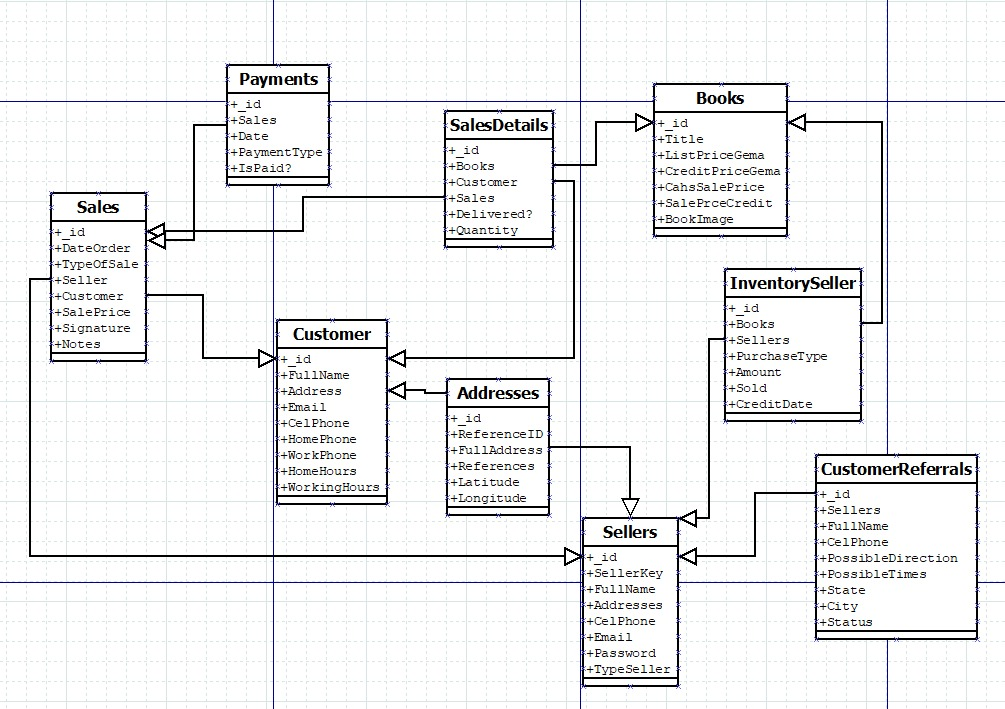
\includegraphics[width=0.8\textwidth]{figures/db_diagrams/DB Diagram.jpg}
	\caption{Diseño de Base de Datos} \label{fig6}
\end{figure}

\subsection{Desarrollo}

La reutilizacion de componentes de software es un proceso mediante el cual se utilizan componentes existentes en el desarrollo de nuevos sistemas o aplicaciones. Los componentes de software reutilizables son aquellos que se han diseñado y desarrollado con el propósito de ser utilizados en diferentes contextos y aplicaciones.

Los componentes identificados en este proyecto para su reutilización a nivel general son los siguientes:
\begin{itemize}
    \item \textbf{Controladores: }Son componentes que encapsulan la lógica de negocio y se comunican con los modelos y las vistas. Estos componentes pueden ser reutilizados a través de diferentes aplicaciones dentro del proyecto, ya que su funcionalidad es independiente de la interfaz de usuario y se define según cómo interactúa con otros componentes.
    \item \textbf{Modelos: }Representan la capa de acceso a datos de la aplicación y encapsulan tanto la estructura de datos como la lógica asociada a la persistencia. Al igual que los controladores, los modelos son componentes reutilizables, ya que encapsulan las funciones y datos comunicandose con otros componentes a través de interfaces.
    \item \textbf{Componentes de la interfaz gráfica: }Los elementos como botones, cajas de texto, etc., pueden ser reutilizados a través de diferentes vistas en la aplicación. Estos componentes encapsulan su funcionalidad y se comunican con otros componentes a través de eventos.
    \item \textbf{Interfaces de datos: }Los servicios web o los servicios REST, encapsulan la funcionalidad de acceso a datos y se comunican con otros componentes a través de interfaces definidas. Estas interfaces pueden ser reutilizadas a través de diferentes aplicaciones dentro del proyecto.
    \item \textbf{Especificaciones: }Definen los requisitos funcionales y no funcionales de la aplicación y pueden ser reutilizadas a través de diferentes etapas del ciclo de vida del software, como el diseño y la implementación.
\end{itemize}   

Estos componentes de rehúso se dividen en base a los niveles de reutilizacion de un proyecto de software y que se aplican a este proyecto de la siguiente manera:

\subsection*{Reutilización a Nivel de Código}

Se refiere a Librerías de funciones, editores, inclusión de ficheros, mecanismos de herencia en POO, componentes, etc.

En este proyecto se aplica la reutilizacion a nivel de codigo en los siguientes componentes:

\subsubsection*{Modelos de Datos Definidos en Clases:}
Estos encapsulan los datos y sus funciones, interactuando con otros componentes mediante su uso en las solicitudes y respuestas HTTP (Ver AdressModel en el Listing \ref{code1}). Son reutilizables al momento de crear una clase para definir un modelo de datos para la aplicación y así gestionar los datos que vengan como respuesta en peticiones HTTP dentro de la aplicación.
\lstinputlisting[caption={Ejemplo de Modelo de Datos},label=code1]{codes/model.dart}

\subsubsection*{Funciones de Peticiones HTTP:}
Estas funciones se encargan de hacer solicitudes HTTP, tanto GET como POST, hacia el servidor. Son reutilizables a través de la aplicación en diferentes secciones que necesiten realizar solicitudes a la API, es decir, al momento de requerir cualquier tipo de información o en el caso de que se requiera enviar información al servidor. Se puede ver reflejado al momento de iniciar sesión o registrarse como se observa en el Listing \ref{code2}, realizar una venta, registrar una referencia, etc. Estas peticiones suelen estar conformadas por información necesaria para la aplicación y alguna de ésta puede ser tomada como otro componente.
\lstinputlisting[caption={Ejemplo de Funciones http},label=code2]{codes/http.dart}

\subsubsection*{Creación de Widgets Personalizados:}
Son componentes de UI que encapsulan funciones y datos específicos. Son reutilizables a través de la aplicación en diferentes pantallas y secciones donde se ocupa un mismo widget y solamente cambie la información de éste, como un icono, el color o el texto dentro del mismo. Es muy útil ya que se evita repetir el código cada vez que se requiera crear un widget con características similares. Los widgets personalizados por lo general tienen componentes sencillos dentro de ellos como texto o iconos, los cuales son tomados en cuenta como otros widgets (ver Listing \ref{code3}).
\lstinputlisting[caption={Ejemplo de Widget Personalizado},label=code3]{codes/widgets.dart}

\subsubsection*{Creación de Pantallas Personalizadas:}
Estas pantallas encapsulan su propia lógica y funcionamiento, interactuando con otros componentes de forma modular. Son reutilizables al momento de crear alguna pantalla que tiene un diseño preestablecido o que se está retomando de alguna otra pantalla pero con algunos elementos diferentes como botones o colores como se observa en el Listing \ref{code4}. Estas pantallas, a su vez, pueden contener componentes adicionales dentro de ellas, ya sea que estén preestablecidos o que se creen al momento de crear la pantalla, de tal forma que tienen la posibilidad de contener otros componentes dentro.
\lstinputlisting[caption={Ejemplo de Pantalla Personalizada},label=code4]{codes/screen.dart}

\subsubsection*{Validaciones de Formularios:}
Estas encapsulan sus propias reglas y su comportamiento, interactuando con otros componentes de la aplicación en el proceso de validación. Son reutilizables en pantallas o secciones de la aplicación donde se necesita validar una información ingresada, como por ejemplo en la validación de las credenciales del usuario (ver Listing \ref{code5}) y al momento de registrar una venta o un crédito.
\lstinputlisting[caption={Ejemplo de validación de Formulario},label=code5]{codes/validacion_form.dart}

\subsubsection*{Snippets y Funciones Prefabricadas:}
Encapsulan lógica y comportamiento específico, interactuando con otros componentes en diferentes secciones y módulos de la aplicación. Son reutilizables al momento de crear nuevas pantallas (ejemplo Listing \ref{code6}), widgets o funciones, dependiendo del resultado o componente que se desea y pueden contener también componentes prefabricados dentro de ellas o algún componente personalizado.
\lstinputlisting[caption={Ejemplo de Funcion Prefabricada},label=code6]{codes/funcion_prefabricada.dart}

\subsubsection*{Funciones de Gestión de Estado:}
Encapsulan el estado de la aplicación, interactuando con otros componentes en diferentes secciones y módulos. Son reutilizables en diferentes contextos que necesiten gestionar el estado de la aplicación, ya sea al momento de obtener la respuesta de una petición HTTP realizada o cuando se requiera actualizar el estado de la aplicación. Estos gestores de estado suelen contener dentro los componentes o funciones que alteran el comportamiento o estado de los mismos (ver Listing \ref{code7}), por lo que en ocasiones requieren ser contemplados dentro de los gestores de estado.
\lstinputlisting[caption={Ejemplo de Funcion de Gestión de Estado},label=code7]{codes/gestion_estado.dart}


\subsection*{Reutilización a Nivel de Diseño}
Consiste en no volver a inventar arquitecturas y utilizar las que están disponibles así como patrones de diseño o de arquitectura.

En proyecto se aplica la reutilizacion a nivel de diseño en los siguientes componentes:

\subsubsection*{Patron Provider (Semejante a Singleton) para la Gestión del Estado:}
Es un patrón de diseño que se utiliza en el desarrollo de software para administrar el estado global de la aplicación de manera eficiente y escalable. Su objetivo principal es proporcionar un flujo de datos constante y actualizado en toda la aplicación, eliminando la necesidad de pasar explícitamente los datos entre los diferentes componentes de la aplicación como se observa en el Listing \ref{code8}. 
\lstinputlisting[caption={Ejemplo de Aplicación de Patron Provider},label=code8]{codes/provider.dart}

\subsubsection*{Elementos Gráficos: }
El objetivo es que estos elementos tengan un aspecto y funcionalidad coherente y consistente en toda la aplicación. Al utilizar componentes, se ahorra tiempo en el desarrollo, se reduce el número de errores y se aumenta la consistencia visual y de interacción en la aplicación. Además, estos componentes pueden ser mejorados y actualizados de forma centralizada, lo que facilita su mantenimiento y evolución.

Ademas, algunos de estos componentes pueden contener otros componentes dentro y también encapsulan funciones de acción o de estado así como datos en algunos casos como pueden ser campos de texto (ver Figura \ref{fig8}) o botones (ver Figura \ref{fig9}) o en el caso de la barra de navegación que contiene las rutas de la aplicación las cuales sirven para comunicarse dentro de la aplicación (ver Figura \ref{fig7}).

\begin{figure}[H]
	\centering\captionsetup{width=0.8\textwidth}
	
\includegraphics[width=0.6\textwidth]{figures/graphic_components/barra_navegacion.png}
	\caption{Barra de Navegación} \label{fig7}
\end{figure}
\begin{figure}[H]
	\centering\captionsetup{width=0.8\textwidth}
	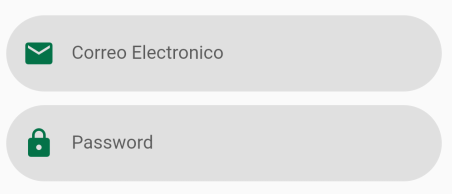
\includegraphics[width=0.6\textwidth]{figures/graphic_components/text_fields.png}
	\caption{Campos de Texto} \label{fig8}
\end{figure}
\begin{figure}[H]
	\centering\captionsetup{width=0.8\textwidth}
	
\includegraphics[width=0.6\textwidth]{figures/graphic_components/button.png}
	\caption{Botones} \label{fig9}
\end{figure}

Algo muy importante a resaltar dentro de los componentes y elementos graficos es el tema de la aplicacion, el cual incluye colores y formas de estos elementos.
La paleta de colores designada para este proyecto (Figura \ref{fig10}) se basa en los colores representativos del club Kerusso, los cuales en su mayoria se encuentras reflejados en su logo.
\begin{figure}[H]
	\centering\captionsetup{width=0.8\textwidth}
	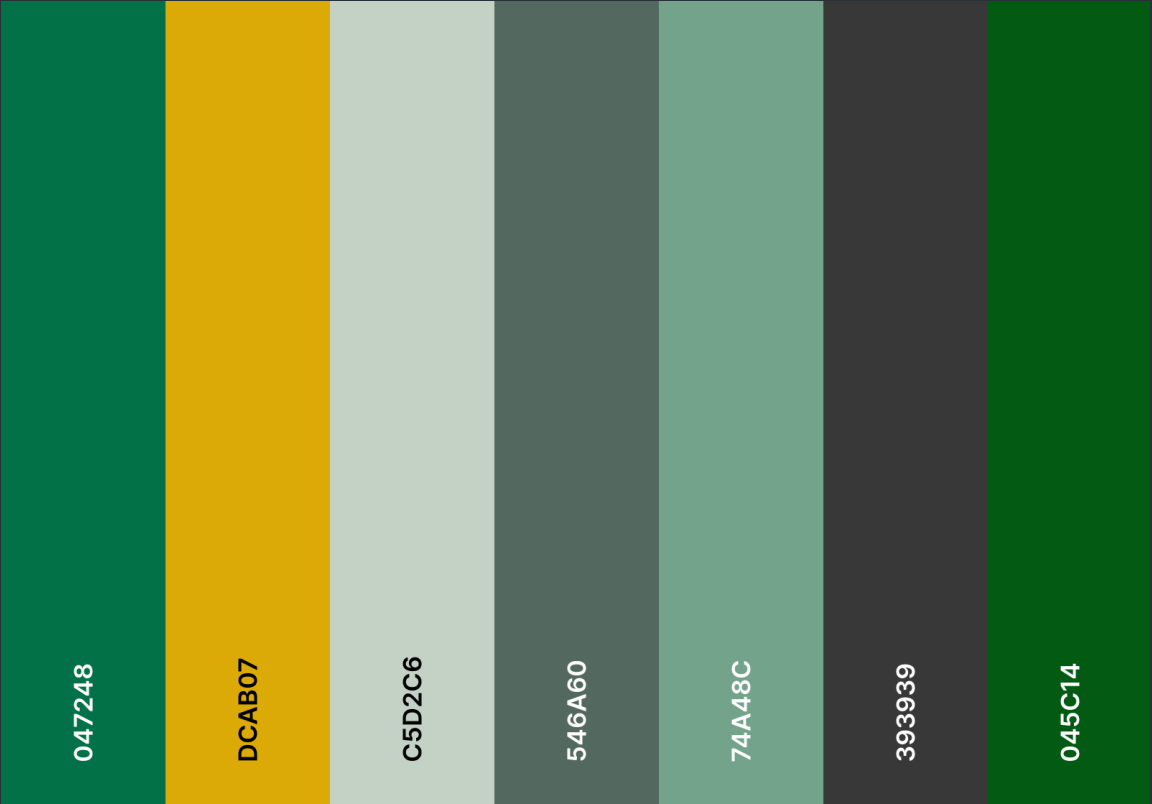
\includegraphics[width=0.6\textwidth]{figures/graphic_components/colors.png}
	\caption{Paleta de Colores} \label{fig10}
\end{figure}

\subsubsection*{Interfaces de Datos}
\subsection*{Reutilizacion a Nivel de Especificaciones y Funciones}
Las especificaciones definen los requisitos funcionales y no funcionales de la aplicación y pueden ser reutilizadas a través de diferentes etapas del ciclo de vida del software, como el diseño y la implementación.
En este proyecto se están reutilizando las siguientes funciones:
\begin{itemize}
    \item Definición de Cliente en Base a una Referencia
    \item Selección de Material
    \item Proceso de Registro de Crédito de Libros y Compras al Contado
    \item Proceso de Registro de Venta
    \item Proceso de Validación de Usuario
\end{itemize}
Como puede observarse, son procesos que derivan de los requerimientos y que cada uno de estos se reutiliza tanto a nivel de funcionalidad como a nivel de interacción con el usuario, ya que son procesos que dependen de otros o que se establecen a partir de información proporcionada por otras partes de la aplicación o por el usuario y que el resultado dependerá también de información ingresada, por lo que su ejecución estará en constante proceso de reutilizacion.
\end{document}